\begin{small}
  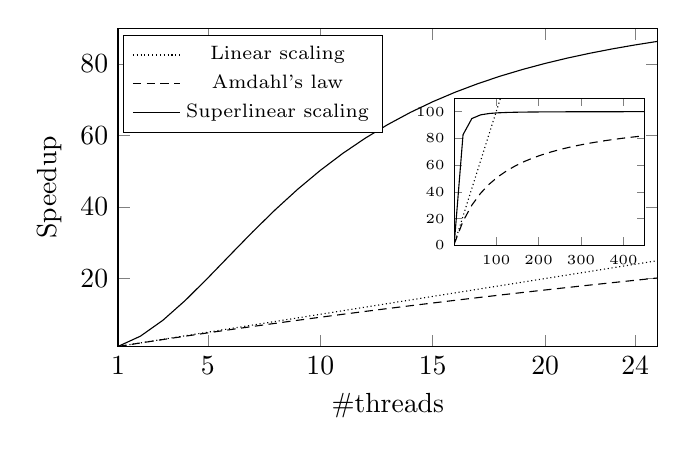
\begin{tikzpicture}[remember picture]
    \begin{axis}[
      width=240pt,
      height=160pt,
      xlabel={\#threads},
      ylabel={Speedup},
      xlabel near ticks,
      ylabel near ticks,
      xmin=1,
      xmax=25,
      ymin=1,
      ymax=90,
      xtick={1,5,10,15,20,24},
      legend style = {
        anchor = north west,
        at = {(rel axis cs:0.01,0.98)},
        font=\scriptsize,
        % draw = none,
      },
      no markers
      ]
      % use TeX as calculator:
      \addplot[domain=1:25,black,densely dotted]{x};
      \addlegendentry{Linear scaling}

      \addplot[domain=1:25,black,densely dashed]{1/(0.01 + (1-0.01)/x)};
      \addlegendentry{Amdahl's law}

      \addplot[domain=1:25,black,solid]{1/(0.01 + (1-0.01)/x^2)};
      \addlegendentry{Superlinear scaling}

      \coordinate (insetPosition) at (rel axis cs:.98,0.23);
      % \addplot[domain=0:15,black,loosely dashed]{1/(0.4 + (1-0.4)/x)};
      % \addlegendentry{Amdahl's law ($\delta=0.4$)}

      % \addplot[domain=0:15,black,loosely dotted]{1/(0.4 + (1-0.4)/x^2)};
      % \addlegendentry{Proposed scaling law for MTF ($\delta=0.4$)}
    \end{axis}
    \begin{axis}[
      at={(insetPosition)},
      anchor={outer south east},
      width=105pt,
      height=85pt,
      tiny,
      % xlabel={\#cores},
      % ylabel={Speedup},
      xmin=1,
      xmax=450,
      ymin=0,
      ymax=110,
      % ytick={1,2,3,4,5},
      no markers]
      \addplot[domain=1:500,black,densely dotted]{x};
      \addplot[domain=1:500,black,densely dashed]{1/(0.01 + (1-0.01)/x)};
      \addplot[domain=1:500,black,solid]{1/(0.01 + (1-0.01)/x^2)};
    \end{axis}
  \end{tikzpicture}
\end{small}

%%% Local Variables:
%%% mode: latex
%%% TeX-master: "../distributed_mrf.tex"
%%% End:
